\chapter{实验数据分析}\label{chap:Epxeriment}

本章首先介绍了微译器的实验环境,在添加指令翻译过程的调试环境。
然后展示了微译器在X86和RISCV上的性能分析,
最后分析了实施的优化方案的效果。

\section{实验环境}

本课题在Gem5模拟器\cite{gem5OriginalPaper}上进行了实验,Gem5是一个广泛使用的开源计算机系统体系结构模拟器,
它具有如下特点:
\begin{itemize}
  \item 开源:Gem5是一个开源项目,每年都会有大量的开发者参与到Gem5的开发中并发布新的版本。
  过去12年间,有超过250名开发者参与到Gem5的开发中,提交了超过7500次的commit\cite{Gem5SimulatorVersion2020}。
  目前最新的版本是v23,也是我们使用的版本。
  \item 广泛使用:Gem5被广泛用于学术界和工业界,用于研究新的计算机体系结构,新的内存层次结构,新的缓存替换算法等。
  \item 周期精确:Gem5是一个周期精确的模拟器,可以模拟CPU的每一个周期,\cite{Butko2012AccuracyEO}表明Gem5与实际硬件的性能差距在5\%以内。
  \item 多架构支持:Gem5支持多种指令集架构,包括X86、RISCV、ARM等,可以方便的进行不同架构的模拟,便于本课题的研究。
  \item 模块化:Gem5的设计是模块化的,分为CPU模块、缓存模块、内存模块等,可以方便的进行模块的替换和扩展。
  \item 高度可配置:Gem5在一次编译后,在动态运行时可以通过配置参数进行不同的配置,例如CPU类型、缓存大小等。
  \item 事件驱动:Gem5是一个事件驱动的模拟器,它将时间的流逝模拟为一系列离散事件,只有在事件发生时才会进行模拟。
  例如在模拟CPU时,只有在取指、译码、执行等事件发生时才会进行慢速模拟,其余时间Gem5会快速跳过,这样可以提高模拟器的效率。
\end{itemize}

Gem5有全系统模拟器和用户空间模拟器两种模式,全系统模拟器可以模拟整个计算机系统,包括CPU、内存、外设等,
用户空间模拟器只模拟用户空间的部分,不模拟内核和硬件,只模拟用户空间的指令执行\cite{gem5OriginalPaper}。
本课题使用\textbf{用户空间}模拟器进行实验,因为本课题主要关注用户态二进制翻译器优化,只翻译用户态的指令,不涉及内核态的指令。

为了和真实的硬件环境更加接近,我们使用了和真实硬件校准过的Intel Haswell X86处理器\cite{haswell_cpu}参数进行模拟,
\cite{akramValidationGem5Simulator2019}校准后的数据表明,Gem5模拟器和真实硬件的性能差距在6\%以内。
我们将这个参数作为\textbf{基准参数},然后在这个基准参数上进行微译器的实验。接下来的性能对比都是相对于这个基准参数进行的。

为了不引入额外的面积、功耗等开销,我们使用同样大小的翻译缓存\textbf{替换}了原有的指令缓存,这样可以保证硬件开销不变。
表\ref{tab:specifications}展示了Gem5的硬件参数。

% https://www.tablesgenerator.com/latex_tables
\begin{table}[ht]
  \centering
  \caption{Gem5硬件参数,其中指令缓存模式为Intel Haswell处理器参数; 翻译缓存模式为微译器参数。
        仅替换了前端的指令缓存,其余参数保持不变。}
  \label{tab:specifications}
  \begin{tabular}{|c|ll|}
  \hline
  \multicolumn{1}{|l|}{}         & \multicolumn{1}{l|}{\textbf{翻译缓存模式}} & \textbf{指令缓存模式} \\ \hline
  \multirow{6}{*}{\textbf{处理器核}} & \multicolumn{1}{l|}{软件动静翻译+融合微码}           & 硬件译码 + RISCV指令    \\ \cline{2-3} 
                                 & \multicolumn{2}{l|}{类型:乱序6发射处理器}                         \\ \cline{2-3} 
                                 & \multicolumn{2}{l|}{译码:每拍6条}                         \\ \cline{2-3} 
                                 & \multicolumn{2}{l|}{主频:3.4GHz}                         \\ \cline{2-3} 
                                 & \multicolumn{2}{l|}{分发:每拍6条微码}                         \\ \cline{2-3} 
                                 & \multicolumn{2}{l|}{发射队列:69条微码}                                 \\ \cline{2-3} 
                                 & \multicolumn{2}{l|}{分支预测:4096项的锦标赛算法}                            \\ \hline
  \multirow{5}{*}{\textbf{\begin{tabular}[c]{@{}c@{}}内存层次\end{tabular}}} &
                    \multicolumn{1}{l|}{
                    \begin{tabular}[c]{@{}l@{}}翻译缓存: 32KB,\\8路组相连,2拍延迟\end{tabular}} &
                    \begin{tabular}[c]{@{}l@{}}指令缓存: 32KB,\\8路组相连,2拍延迟\end{tabular} \\ \cline{2-3} 
                                 & \multicolumn{2}{l|}{数据缓存: 32KB,8路组相连,2拍延迟}                    \\ \cline{2-3} 
                                 & \multicolumn{2}{l|}{二级缓存: 256KB,8路组相连,12拍延迟}                \\ \cline{2-3} 
                                 & \multicolumn{2}{l|}{三级缓存: 8MB,16路组相连,36拍延迟}                 \\ \cline{2-3} 
                                 & \multicolumn{2}{l|}{内存: 4GB,DDR3-1600, 30ns延迟}                     \\ \hline
  \end{tabular}
  \end{table}

\section{测试程序}

本课题使用了Coremark,SPEC CPU 2000测试集作为测试程序。
Coremark 是一个小型的基准测试程序,主要用于测试嵌入式系统的性能,它包括了一些基本的计算、控制流、内存访问等操作,可以通过参数指定循环次数来控制运行时间。
SPEC CPU 2000测试集是一个通用的测试CPU性能的测试集,包括了12个整数测试程序和14个浮点测试程序,是一个较为完备的测试集,本机运行时间在几分钟量级。

由于Gem5模拟器性能开销较大,在使用用户态模拟、乱序处理器模型的配置下,相对于本机运行时间,Gem5平均慢1万倍,这意味着一个在本机上运行1秒的程序,在Gem5上需要运行3小时。
因此选择SPEC 2000 test测试集来缩短实验时间,
而Coremark测试集设置循环1000次来控制运行时间,
所有测试程序在Gem5模拟器上运行的时间均控制在几分钟到几小时之间,这样方便我们进行实验。

测试程序使用riscv64-linux-gnu-gcc交叉编译器编译到RISCV架构上,gcc 版本为12.3,
编译参数均为\texttt{-O3 --static}静态编译,SPEC程序还有其默认的编译参数。

\section{调试环境}

为了保证整个微译器的正确性,需要好的测试集和调试环境。

对于测试集,我们使用了单元测试、集成测试、性能测试等多种测试手段,保证了翻译器的正确性。
单元测试用于测试软件端翻译器的正确性,集成测试用于测试微译器在运行小型测试程序时的正确性,性能测试用于测试微译器在运行大型测试程序时的性能。
\begin{itemize}
\item 单元测试: 选择了riscv-tests\cite{riscv-tests}和riscv-arch-tests\cite{riscv-arch-tests},两者均使用汇编语言编写,用于测试单条RISCV指令能否正确翻译运行,
前者对RISCV IMAFD每条指令均有10余个测试用例,后者能生成数百个整数指令的随机测试用例。
\item 集成测试: 使用了手写的C语言程序,用于测试微译器在运行小型测试程序时的正确性,例如能否正确的初始化栈信息、能否正确处理系统调用等。
\item 性能测试: 使用了Coremark和SPEC 2000 test测试集,用于测试微译器在运行大型测试程序时的性能。
\end{itemize}

如果测试程序出现了错误,可以通过调试环境来定位错误。
由于Gem5上无法直接运行GDB调试器,本课题通过打印指令执行信息、打印寄存器信息等方式来定位错误。
对于含有错误的微译器,需要和标准正确的Gem5模拟器进行对比,找出错误的原因。
标准正确的Gem5模拟器是指没有任何修改的、配置为RISCV架构的Gem5模拟器,它能直接硬件译码运行RISCV程序。
通过在Gem5模拟器上添加了打印所有整数、浮点寄存器信息的功能,当指令执行流比对不一致时,可以通过打印寄存器信息来定位错误。

% \section{微译器在X86上性能分析}

% 图\ref{img:ucache_ipc}展示了微译器在X86上SPEC 2017上的翻译运行结果,相对于未修改过的X86指令缓存模式进行了归一化。
% 可以看到,微译器在SPEC 2017上的性能接近于原生运行,平均性能为92.3\%,并且一大半的浮点型测试集的性能损失在1\%以内。

% \begin{figure}[!htbp]
%   \centering
%   \includegraphics[width=1\linewidth]{./plot_pdf/ucache_ipc.pdf}
%   \caption{微译器运行SPEC CPU 2017的性能,相对于未修改过的X86指令缓存模式进行了归一化。}
%   \label{img:ucache_ipc}
% \end{figure}

% 图\ref{img:new_cache_miss}展示了微译器在X86上SPEC 2017上的每千条指令的未命中次数(MPKI),
% 根据计算,每千条指令的未命中次数和性能之间的皮尔森相关系数为-0.93,说明未命中次数和性能之间存在很强的负相关性。
% 这也说明了微译器的性能主要受到了未命中次数的影响。

% \begin{figure}[!htbp]
%   \centering
%   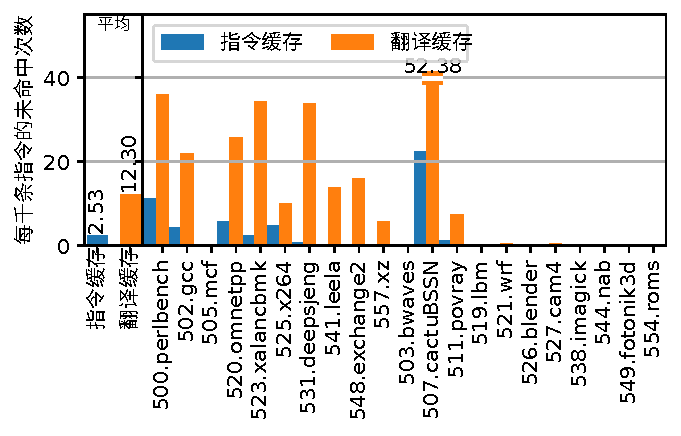
\includegraphics[width=1\linewidth]{./plot_pdf/new_cache_miss.pdf}
%   \caption{微译器运行SPEC CPU 2017的每千条指令的未命中次数。}
%   \label{img:new_cache_miss}
% \end{figure}

% \begin{table}[]
%   \centering
%   \caption{
%     微译器运行CoreMark测试集的性能对比。
%   }
%   \label{tab:coremark}
%   \begin{tabular}{llll}
%   \rowcolor[HTML]{FFCE93} 
%                & x86\_raw & x86\_ucache & riscv\_ucache \\
%   Insts        & 34655642 & 34655642    & 35899262      \\
%   Cycles       & 26220774 & 26301941    & 28797485      \\
%   IPC          & 1.321686 & 1.317608    & 1.246611      \\
%   IPC/IPC\_raw & 100\%    & 99.69\%     & 94.32\%      
%   \end{tabular}
%   \end{table}

% 我们在X86上运行了CoreMark测试集,相对于普通的ICache配置项,也就是没有任何修改的运行X86程序,
% 我们的微译器在翻译运行的性能为99\%,对应的每千条指令的未命中次数为0.9,也符合上述规律,
% 这主要在于程序的取指行为,CoreMark程序中主要为核心循环计算,时间局部性和空间局部性都很好,因此未命中次数较少,性能也较好。
% 即便经过微译器的预翻译文件膨胀,也能够在X86上保持较好的性能。

% 我们在RISCV上运行了CoreMark测试集,得到了性能为94\%,对应的每千条指令的未命中次数为1.1,也符合上述规律。

% RISCV 相对于X86的CoreMark 还有一定的性能差距,主要由于还没有添加硬件返回栈支持,导致对于函数调用的支持不够完善,因此性能有所下降。

% 同时RISCV目前对于压缩指令支持还不够完善,导致翻译出来的微码编码较长,导致AOT文件相对更大,也会导致性能下降。


\section{性能分析}
由于Gem5的模拟器的性能开销较大,我们选择了SPEC CPU 2000 test测试集作为测试基准。
SPEC CPU 2000 test测试集包括了12个整数测试程序和14个浮点测试程序,是一个较为完备的测试集。
目前已经成功运行了8个整数测试程序,剩下的整数测试程序由于指令翻译的问题暂时无法运行,目前还在修复中,浮点测试程序还没有测试。

如图\ref{img:ipc}所示,我们的微译器在运行SPEC CPU 2000 test测试集时(这里只关注RISCV程序),总共有三个测试配置,分别为:
\begin{itemize}
  \item 使用指令缓存(基准参数):CPU没有修改,通过内存层次、多级缓存和指令缓存,硬件译码并运行RISCV程序。
  \item 使用翻译缓存:软件端二进制翻译器把RISCV指令翻译为融合微码,CPU通过内存层次、多级缓存和微码缓存,硬件运行融合微码。
  \item 使用翻译缓存并有所有优化:在上一个配置基础上,开启了所有优化选项,让一行微码行中存储微码指令数目变多了,减少翻译缓存缺失率。
\end{itemize}

我们以指令每周期数(IPC)作为性能指标,IPC越大,性能越好。以指令缓存模式为基准性能,翻译缓存模式的性能为基准性能的百分比,
并分别测量关闭优化以及开启所有优化的性能。
如图\ref{img:ipc}所示,我们的微译器在运行SPEC2000 整数测试集时,性能表现如下:
在不开启任何优化的情况下,性能表现在加上微码缓存后,性能为原生性能87.8\%,其中主要是176.gcc和186.crafty两个测试程序性能下降较多;
这是由于这两个测试程序代码循环较少,时间局部性较差,指令代码较多,导致了大量的缓存缺失;
而对于其他的几个测试程序,性能大多在90\%以上,说明这些程序的时间局部性较好,性能下降较少,微译器的性能表现较好。

在开启所有优化后,性能为原生性能的94\%,性能提升了6\%,说明优化方案的效果较好。
对于176.gcc和186.crafty两个测试程序,性能提升较多,分别为20\%和24\%。
下一小节将对优化方案进行分析。


\begin{figure}[!htbp]
  \centering
  \includegraphics[width=0.8\linewidth]{./plot/ucache_ipc.pdf}
  \caption{SPEC2000整数性能对比图。}
  \label{img:ipc}
\end{figure}

如图\ref{img:miss_rate}所示,我们的微译器在运行SPEC2000 整数测试集时,翻译缓存缺失率表现如下:
未开启优化时,缓存缺失率平均为2.3\%,其中最高的为gcc和crafty测试程序,缓存缺失率为7.7\%和9.2\%;这与性能表现相符,缓存缺失率越高,性能越低。
开启所有优化后,缓存缺失率平均为0.6\%,下降了1.7\%,说明优化方案的效果较好。
经过计算,缓存缺失率和性能之间的皮尔森相关系数为-0.91,说明缓存缺失率和性能之间存在很强的负相关性。目前的性能下降主要受到了未命中次数的影响。

\begin{figure}[!htbp]
  \centering
  \includegraphics[width=0.8\linewidth]{./plot/miss_rate.pdf}
  \caption{SPEC2000整数测试下缓存缺失率。}
  \label{img:miss_rate}
\end{figure}

如图\ref{img:ipc_fp}所示,我们的微译器在运行SPEC2000 浮点测试集时,性能表现如下:
在不开启任何优化的情况下,性能表现在加上微码缓存后,性能为原生性能的96.5\%;
在开启所有优化后,性能为原生性能98.2\%,性能提升了1.7\%。
这说明无论是否开启优化,微译器对于浮点性能表现较好。


\begin{figure}[!htbp]
  \centering
  \includegraphics[width=0.8\linewidth]{./plot/ucache_ipc_fp.pdf}
  \caption{SPEC2000浮点性能对比图。}
  \label{img:ipc_fp}
\end{figure}


\section{优化方案分析}